% !TeX root = vpl.tex

\chap{Cambiare colore}\label{ch.colors}

\sect{Colorare}

Obiettivo di questo capitolo è creare un programma che visualizzi due diversi colori nella parte superiore del robot Thymio quando i pulsanti anteriore e posteriore vengono toccati, e altri due colori da visualizzare nella parte inferiore del robot
quando vengono toccati il pulsanti destro e sinistro.

{\raggedleft \hfill file di programma \bu{colors.aesl}}

Abbiamo bisogno di quattro coppie di eventi-azione.
Ci sono quattro eventi---toccare i
quattro pulsanti---e un'azione Colore è associata a ogni evento. Notare la
differenza tra i blocchi di azione \blksm{action-colors-up-white} e
\blksm{action-colors-down-white}. Il primo blocco cambia colore
visualizzato sulla parte superiore del robot, mentre il secondo cambia il colore sulla
parte inferiore del robot. Il blocco per la parte inferiore ha due segni neri
che rappresentano le ruote.

Questo programma è mostrato in \cref{fig.colors-a}

Quali colori vengono visualizzati? Nelle prime tre azioni, il cursore per
un colore viene spostato sul bordo destro e visualizzato, mentre i cursori
per gli altri due colori vengono spostati verso il bordo sinistro e quindi non sono mescolati. Pertanto, queste azioni mostrano i colori puri rosso, blu e verde,
rispettivamente. L'azione associata al tasto sinistro mescola rosso e verde
dando giallo .
Si può vedere che lo sfondo dell'azione cambia colore a seconda della
posizioni dei cursori; Lo sfondo mostra di quale colore il vostro Thymio si illuminerà.

Esegui il programma (icona \blksm{run}) e controlla che toccando i tasti cambi il colore del robot.
\Cref{fig.front} mostra il Thymio di colore rosso
nella parte superiore e \cref{fig.bottom} mostra il colore verde sulla parte
inferiore.

\exercisebox{\thechapter.1}{
Sperimentate con i cursori per vedere quali colori vengono visualizzati
}

\trickbox[Informazione]{
\gr{color-cubes-en}{1}
Miscelando rosso, verde e blu puoi fare qualsiasi altro colore!
}

\sect{Spegnere la luce}

Cerchiamo di modificare il programma in modo che le luci vengano spente quando si tocca il
pulsante centrale. Abbiamo bisogno di due coppie di eventi-azione, uno per spegnere la luce superiore e l'altra per spegnere la luce inferiore.
Spostando i cursori nel blocco di azione colore a sinistra, come in \cref{fig.colors-b}, senza colori vengono visualizzati e la spia si spegne.
L'\emph{evento è lo stesso in entrambe le coppie}---toccare il pulsante centrale---ma
le \emph{azioni sono diverse}---spegnere la luce superiore o inferiore.

Non dimenticare di cliccare sull'icona \blksmpure{run} per eseguire il programma.
In futuro, non ripeteremo più di fare clic su questa icona per eseguire un programma.

\vfill

\importantbox[Coppie evento-azione multiple]{
\begin{itemize}[noitemsep,nosep,leftmargin=*]
\item Quando si esegue un programma, tutte le coppie evento-azione del programma
sono considerate.
\item E'possibile che per diverse coppie vi sia lo stesso evento
purchè siano diversi blocchi azione associati.
\item Se l'evento e il blocco di azione sono identici in più coppie, VPL mostrerà un messaggio di errore (zona 3 in \cref{fig.vplgui}).
Non sarai in grado di eseguire il programma fino a quando ci sono errori.
\end{itemize}
}

\begin{figure}
    \centering
    \subfigure[Cambiare colore quando si tocca un bottone]{
		\label{fig.colors-a}
		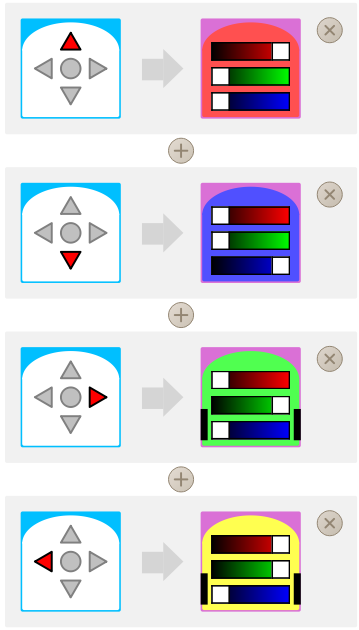
\includegraphics[width = 0.4\textwidth]{colors1}
	}
	\hspace{1.5cm}
    \subfigure[Spegenere la luce quando si tocca un bottone]{
		\label{fig.colors-b}
		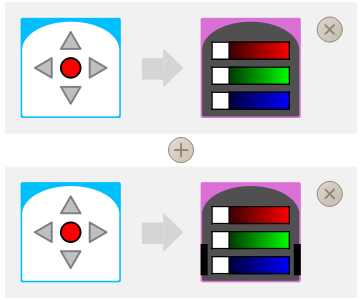
\includegraphics[width = 0.4\textwidth]{colors2}
	}
    \caption{Giocare con le luci di Thymio}
    \label{fig.colors}
\end{figure}
